\subchapter{Accessing Hardware Devices}
{Objective: learn how to access hardware devices and declare new ones.}

\section{Goals}

Now that we have access to a command line shell thanks to a working root
filesystem, we can now explore existing devices and make new ones
available. In particular, we will make changes to the Device Tree
and compile an out-of-tree Linux kernel module.

\section{Setup}

Go to the \code{$HOME/__SESSION_NAME__-labs/hardware} directory,
which provides useful files for this lab.

However, we will go on booting the system through NFS, using the
root filesystem built by the previous lab.

\section{Exploring /dev}

Start by exploring \code{/dev} on your target system. Here are a few
noteworthy device files that you will see:

\begin{itemize}
 \item {\em Terminal devices}: devices starting with \code{tty}.
       Terminals are user interfaces taking text as
       input and producing text as output, and are typically used by
       interactive shells. In particular, you will find
       \code{console} which matches the device specified through
       \code{console=} in the kernel command line. You will also find
       the {\tt \ttyname} device file.
 \item {\em Pseudo-terminal devices}: devices starting with \code{pty},
       used when you connect through SSH for example. Those are virtual
       devices, but there are so many in \code{/dev} that we wanted
       to give a description here.
 \item {MMC device(s) and partitions}: devices starting with
       \code{mmcblk}. You should here recognize the MMC device(s)
       on your system and the associated partitions.
 \item If you have a real board (not QEMU) and a USB stick, you could
       plug it in and if your kernel was built with USB host and mass
       storage support, you should see a new \code{sda} device appear,
       together with the \code{sda<n>} devices for its partitions.
\end{itemize}

Don't hesitate to explore \code{/dev} on your workstation too
and ask any questions to your instructor.

\section{Exploring /sys}

The next thing you can explore is the {\em Sysfs} filesystem.

A good place to start is \code{/sys/class}, which exposes devices
classified by the kernel frameworks which manage them.

For example, go to \code{/sys/class/net}, and you will see all the
networking interfaces on your system, whether they are internal,
external or virtual ones.

Find which subdirectory corresponds to the network connection
to your host system, and then check device properties such as:
\begin{itemize}
   \item \code{speed}: will show you whether this is a gigabit
         or hundred megabit interface.
   \item \code{address}: will show the device MAC address. No
	 need to get it from a complex command!
   \item \code{statistics/rx_bytes} will show you how many bytes
	 were received on this interface.
\end{itemize}

Don't hesitate to look for further interesting properties by yourself!

Next, you can now explore all the buses (virtual or physical) available
on your system, by checking the contents of \code{/sys/bus}.

In particular, go to \code{/sys/bus/mmc/devices} to see all the
MMC devices on your system. Go inside the directory for the first device
and check several files (for example):

\begin{itemize}
\item \code{serial}: the serial number for your device.
\item \code{preferred_erase_size}: the preferred erase block for your
      device. It's recommended that partitions start at multiples of this
      size.
\item \code{name}: the product name for your device. You could display
      it in a user interface or log file, for example.
\item \code{date}: apparently the manufacturing date for the device.
\end{itemize}

Don't hesitate to spend more time exploring \code{/sys} on your system
and asking questions to your instructor.

\section{Driving GPIOs}

At this stage, we can only explore GPIOs through the legacy interface
in \code{/sys/class/gpio}, because the {\em libgpiod} interface
commands are provided through a dedicated project which we have to
build separately, and {\em Busybox} does not provide a
re-implementation for the {\em libgpiod} tools. In a later lab, we
will build {\em libgpiod} tools which use the modern
\code{/dev/gpiochipX} interface.

The first thing to do is to enable this legacy interface by enabling
\kconfig{CONFIG_GPIO_SYSFS} in the kernel configuration.
To do so, in recent Linux kernel versions the \kconfig{CONFIG_EXPERT}
needs to be enabled to have access to some legacy options and in our
case to \kconfig{CONFIG_GPIO_SYSFS}.

Also make sure {\em Debugfs} is enabled (\kconfig{CONFIG_DEBUG_FS} and
\kconfig{CONFIG_DEBUG_FS_ALLOW_ALL}).

Once the new kernel is up, the first thing to do is to mount
the {\em Debugfs} filesystem:

\begin{bashinput}
# mount -t debugfs debugfs /sys/kernel/debug/
\end{bashinput}

Then, you can check information about available GPIOs banks and which
GPIOs are already in use:

\begin{bashinput}
# cat /sys/kernel/debug/gpio
\end{bashinput}

We are going to use one of the EXPI connector of the board,

Take one of the F-F breadboard wires provided by your instructor and:
\begin{itemize}
  \item Connect one end to the \code{Pin 40} of the \code{EXPI} connector
  \item Connect the other end to the \code{GND} pin of the \code{EXPI} connector
\end{itemize}

\begin{center}
  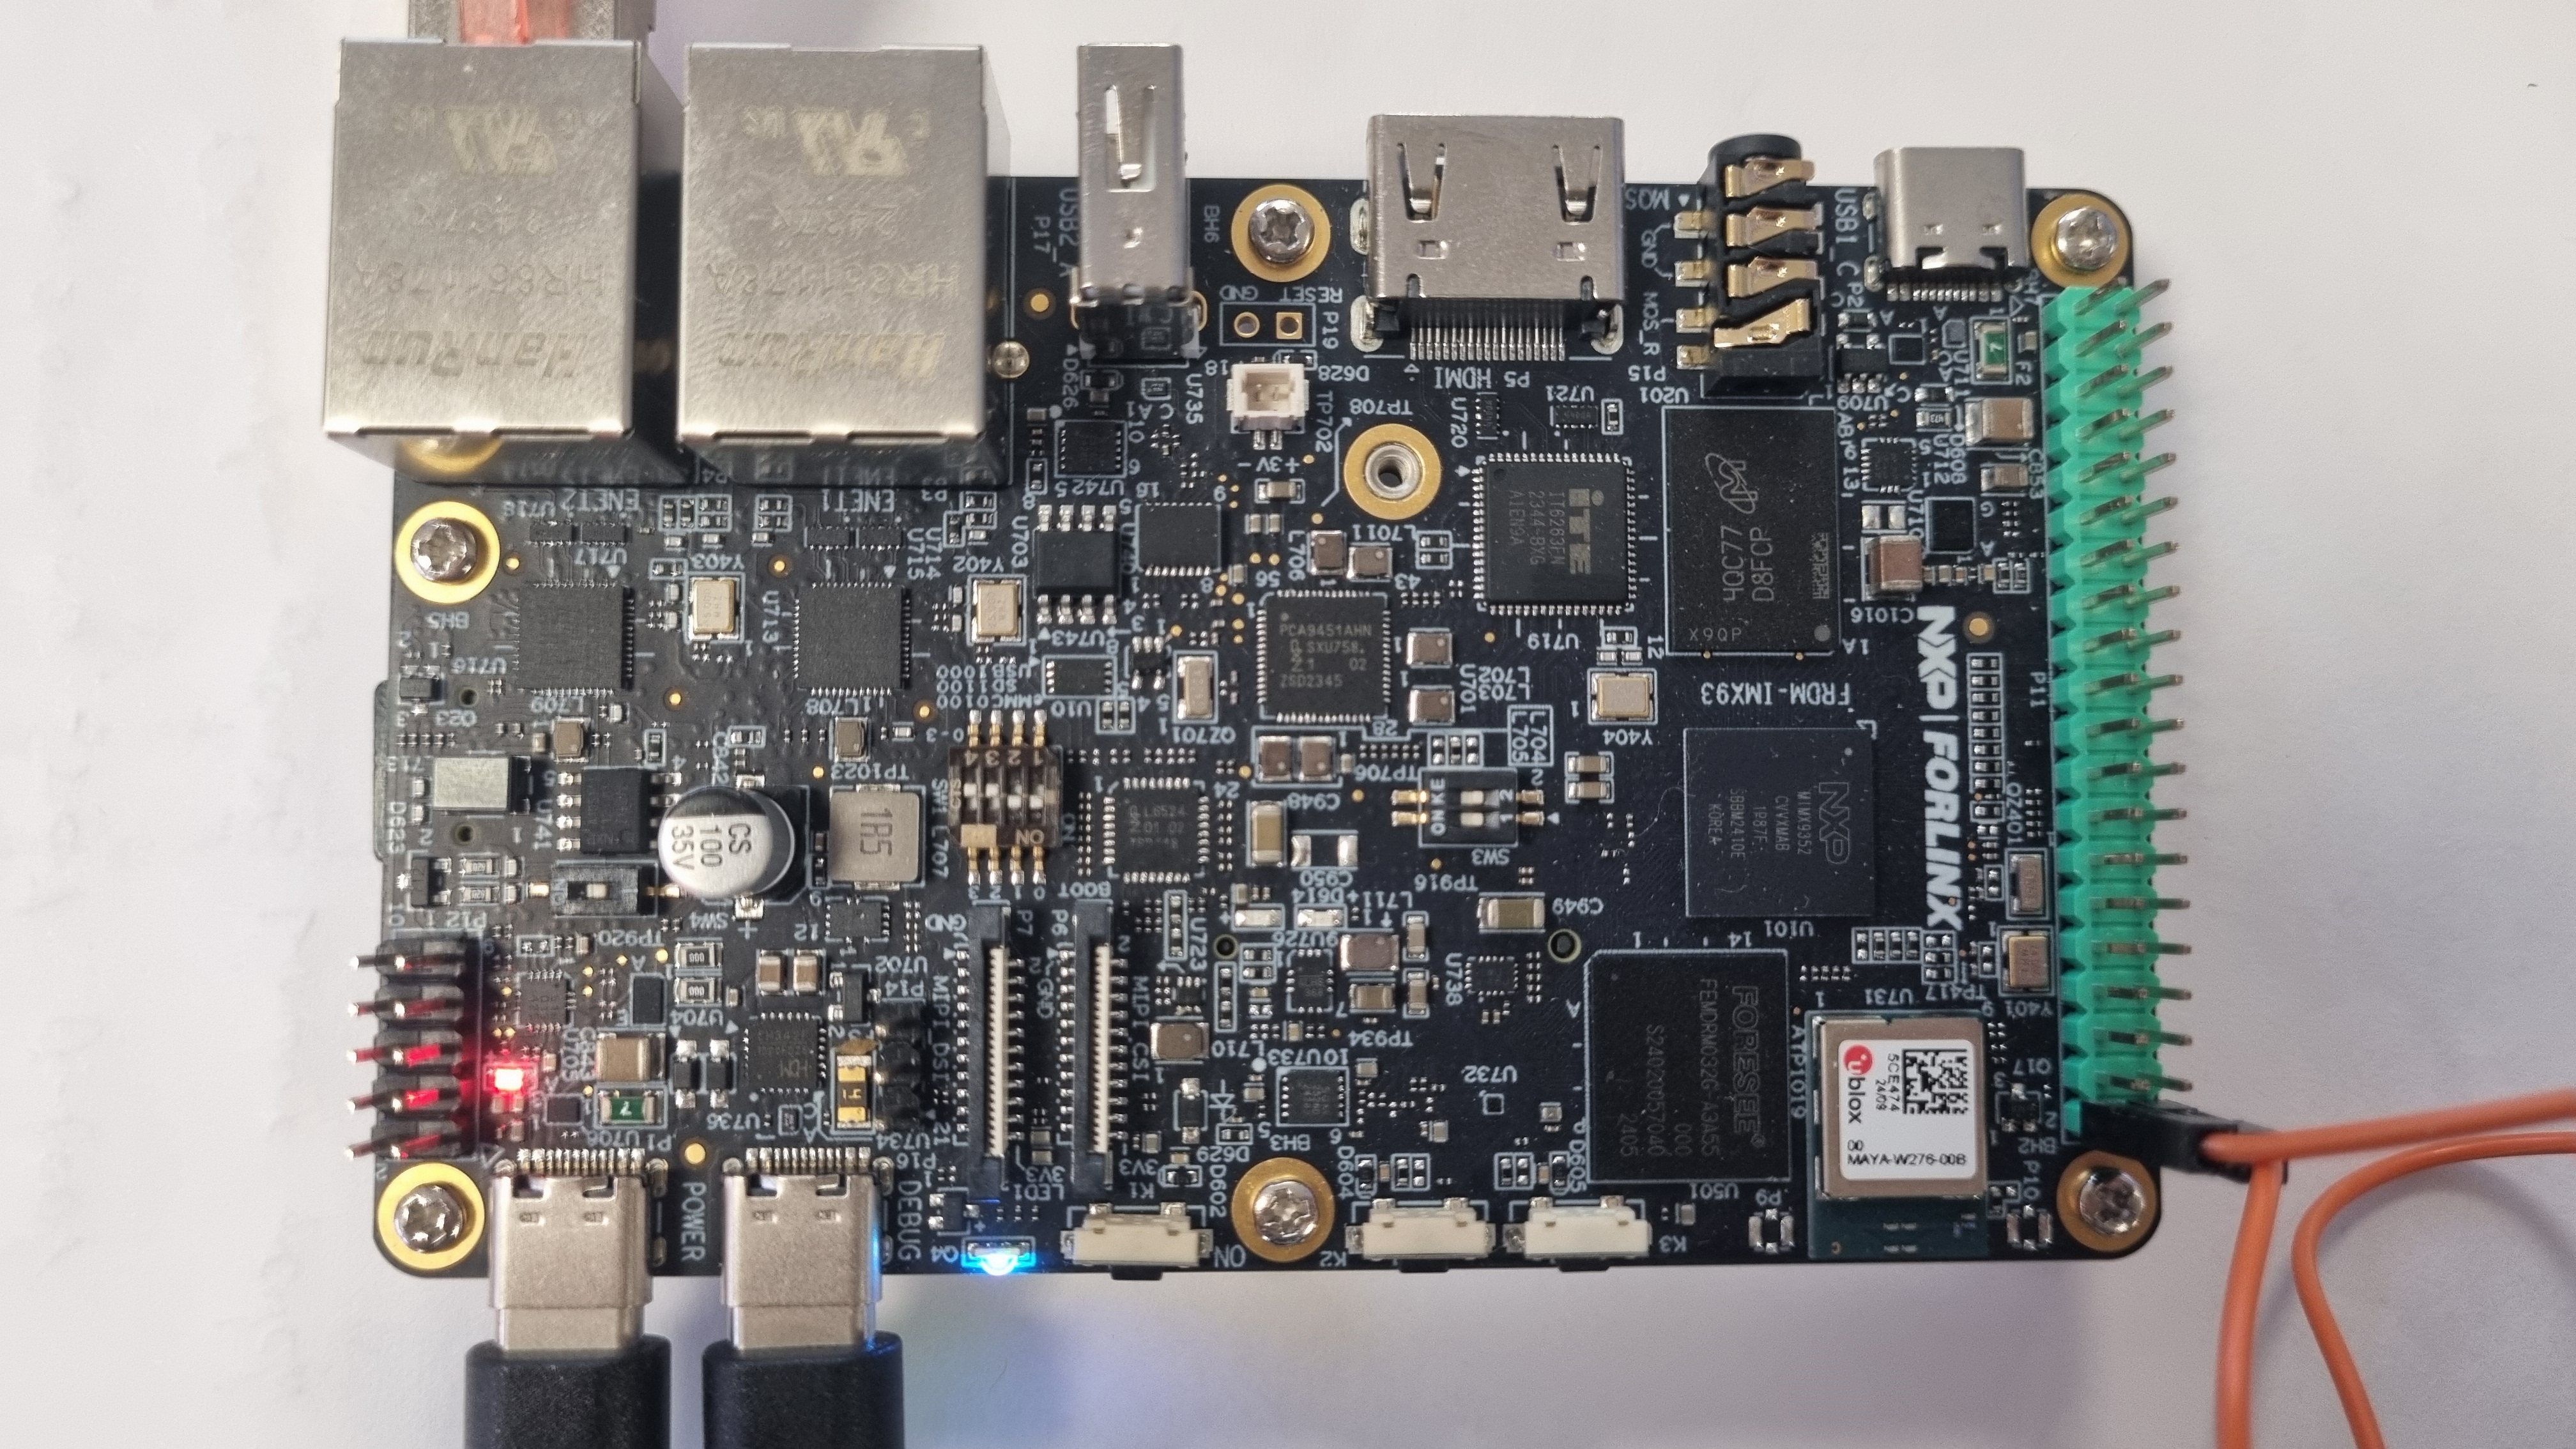
\includegraphics[width=0.5\textwidth]{labs/sysdev-accessing-hardware-imx93-frdm/imx93-frdm-connect-gpio.jpg}
\end{center}

If you look at the {\em IOMUXC} section (§27.3.1.26) of the IMX93 reference manual
\footnote{https://www.nxp.com/docs/en/reference-manual/IMX93RM.pdf}, you will
see that the GPIO\_IO21 PAD is tied to the 21th GPIO of the GPIO2 controller.
In the same document, in the {\em GPIO} section (§28.7.1.1), you'll find the location
of this GPIO controller's registers: 0x43810000.
Then \inlinebash{ls -l /sys/class/gpio} shows the available GPIO controllers and the
device-tree nodes they're tied to. We see that the GPIO controller linked to the
0x43810000 address is called gpiochip512, meaning that its 21th GPIO will be
512 + 21 = 533.

So let's enable this GPIO:

\begin{bashinput}
# cd /sys/class/gpio
# echo %\gpionum% > export
\end{bashinput}

If indeed the pin is still available, this should create a new
{\tt \gpioname} file in \code{/sys/class/gpio}.

We can now configure this pin as input:

\begin{bashinput}
# echo in > %\gpioname%/direction
\end{bashinput}

And check its value:

\begin{bashinput}
# cat %\gpioname%/value
0
\end{bashinput}

The value should be \code{0} as the pin is connected to a ground level.

Now, let's connect our GPIO pin to the \code{+3.3V} pin.

Let's check the value again:

\begin{bashinput}
# cat %\gpioname%/value
1
\end{bashinput}

Note that you could also configure the pin as output and drive it through
the same \code{value} file.

Before moving on to the next section, you can also check
\code{/sys/kernel/debug/gpio} again, and see that {\tt gpio-\gpionum} is now
in use, through the sysfs interface, and is configured as an input pin.

When you're done, you can see your GPIO free:

\begin{bashinput}
# echo %\gpionum% > unexport
\end{bashinput}

\section{Customizing the Device Tree}

\subsection{Driving LEDs}

First, make sure your kernel is compiled with
\kconfigval{CONFIG_LEDS_CLASS}{y}, \kconfigval{CONFIG_LEDS_GPIO}{y}
and \kconfigval{CONFIG_LEDS_TRIGGER_TIMER}{y}.

The \code{/sys/class/leds} folder is empty because no LEDs are known by the
Linux kernel so far.

We're going to start customizing our device-tree to drive the LEDs available
on the FRDM. The FRDM-IMX93 Board User Manual (UM12181) gives details about an
RGB LED: LED1. It's composed of three coloured LEDs, each of them is driven by
a GPIO, let's describe them in the device-tree.

We could modify the \kfile{arch/arm64/boot/dts/freescale/imx93-11x11-frdm.dts}
file for our board, but that's not a very good idea as this file is
maintained by the kernel developers. The changes that you make could
collide with future changes made by the maintainers for this file.

A more futureproof idea is to create a new device-tree file which
includes the standard one, and adds custom definitions. So, create a
new \code{arch/arm64/boot/dts/freescale/imx93-11x11-frdm-custom.dts} file
containing:

\begin{verbatim}
/dts-v1/;
#include "imx93-11x11-frdm.dts"

/ {
        leds {
                compatible = "gpio-leds";
                red: led-0 {
                        label = "red";
                        gpios = <&gpio2 13 GPIO_ACTIVE_HIGH>;
                        default-state = "off";
                };
                green: led-1 {
                        label = "green";
                        gpios = <&gpio2 4 GPIO_ACTIVE_HIGH>;
                        default-state = "off";
                };
                blue: led-2 {
                        label = "blue";
                        gpios = <&gpio2 12 GPIO_ACTIVE_HIGH>;
                        default-state = "off";
                };
        };
};

\end{verbatim}

As you can see, it's also possible to include \code{dts} files, and not
only \code{dtsi} ones.

Modify the \kfile{arch/arm64/boot/dts/freescale/Makefile} file to add your custom
device-tree, and then have it compiled (\code{make dtbs}).

Reboot your board with the update.

Let's control the blue led. Go into the directory for this LED, and check its
trigger (what routine is used to drive its value):

\begin{bashinput}
# cd /sys/class/leds/blue/
# cat trigger
\end{bashinput}

As you can see, there are many triggers to choose from, currently none is
selected.

You can directly control the LED through the \code{brightness} file:

\begin{bashinput}
# echo 1 > brightness
# echo 0 > brightness
\end{bashinput}

You could also use the \code{timer} trigger to light the LED
with specified time on and time off:

\begin{bashinput}
# echo timer > trigger
# echo 10 > delay_on
# echo 200 > delay_off
\end{bashinput}

\subsection{Managing the I2C buses and devices}

The next thing we want to do is connect an Nunchuk joystick
to an I2C bus on our board. The I2C bus is very frequently used
to connect all sorts of external devices. That's why we're covering
it here.

First, let’s see which I2C buses are already enabled:
\begin{bashinput}
# i2cdetect -l
i2c-1	i2c       	44350000.i2c                    	I2C adapter
i2c-2	i2c       	42530000.i2c                    	I2C adapter
i2c-0	i2c       	44340000.i2c                    	I2C adapter
\end{bashinput}

If we look again at the IMX93 reference manual (§60.7.1), we can see that
\code{0x44340000} is the address of the LPI2C1 controller, \code{0x44350000} is
the address of the LPI2C2 controller, and finally, \code{0x42530000} the address
of the LPI2C3 controller.

Let's check the devices present on the i2c-1 bus:

\begin{verbatim}
# i2cdetect -r 1
i2cdetect: WARNING! This program can confuse your I2C bus
Continue? [y/N] y
     0  1  2  3  4  5  6  7  8  9  a  b  c  d  e  f
00:          -- -- -- -- -- -- -- -- -- -- -- -- -- 
10: -- -- -- -- -- -- -- -- -- -- -- -- -- -- -- -- 
20: -- -- UU -- -- UU -- -- -- -- -- -- -- -- -- -- 
30: -- -- -- -- -- -- -- -- -- -- -- -- -- -- -- -- 
40: -- -- -- -- -- -- -- -- -- -- -- -- -- -- -- -- 
50: 50 -- -- -- -- -- -- -- -- -- -- -- -- -- -- -- 
60: -- -- -- -- -- -- -- -- -- -- -- -- -- -- -- -- 
70: -- -- -- -- -- -- -- -- 
\end{verbatim}

Three devices are detected:
\begin{itemize}
\item Two at address \code{0x22} and \code{0x25}, indicated by \code{UU}. Here
  \code{U} stands for 'Under Use' meaning that each of these devices is bound
  to a driver.
\item One other devices at addresses \code{0x50}. No \code{UU} here: the device
  isn't bound to any driver.
\end{itemize}

We are now going to use the \busname\ bus to connect the Nunchuk. Its SDA and SCL
signals are connected to pins 3 and 5 of the EXPI connector (cf the EXPI table
in the GPIO section above).

Fortunately, this bus is already defined in one of the files included in our
device-tree: \kfile{arch/arm64/boot/dts/freescale/imx91_93_common.dtsi}.
Look by yourself in this file, you will find the description under the
\code{lpi2c4} node. As often in .dtsi files, the \code{status} property is set
to \code{disabled}, that's why the bus doesn't appear on our system. So let's
overwrite this \code{status} property by adding the following node to our
custom device-tree:

\begin{verbatim}
&lpi2c4 {
        status = "okay";
};
\end{verbatim}

Rebuild the device-tree and boot again the kernel with the new one, you should
now see one more I2C bus:

\begin{bashinput}
# i2cdetect -l
i2c-3	i2c       	42540000.i2c                    	I2C adapter
i2c-1	i2c       	44350000.i2c                    	I2C adapter
i2c-2	i2c       	42530000.i2c                    	I2C adapter
i2c-0	i2c       	44340000.i2c                    	I2C adapter
\end{bashinput}

Let's check the devices present on our new bus with \inlinebash{i2cdetect -r 3}

You will see that the command will run very slowly because of failing to connect
to the bus. That’s because the corresponding signals are not exposed yet to the
outside connectors through pin muxing.

Let's add the relevant pinmux configuration in our device-tree:

\begin{verbatim}
/dts-v1/;
#include "imx93-11x11-frdm.dts"

/ {
        leds {
                compatible = "gpio-leds";
                red: led-0 {
                        label = "red";
                        gpios = <&gpio2 13 GPIO_ACTIVE_HIGH>;
                        default-state = "off";
                };
                green: led-1 {
                        label = "green";
                        gpios = <&gpio2 4 GPIO_ACTIVE_HIGH>;
                        default-state = "off";
                };
                blue: led-2 {
                        label = "blue";
                        gpios = <&gpio2 12 GPIO_ACTIVE_HIGH>;
                        default-state = "off";
                };
        };
};

&iomuxc {
        pinctrl_lpi2c4_expi: lpi2c4grp {
                fsl,pins = <
                        MX93_PAD_GPIO_IO03__LPI2C4_SCL 0x40000B9E
                        MX93_PAD_GPIO_IO02__LPI2C4_SDA 0x40000B9E
                >;
        };
};


&lpi2c4 {
        pinctrl-names = "default";
        pinctrl-0 = <&pinctrl_lpi2c4_expi>;
        status = "okay";
};
\end{verbatim}

Run again the \code{i2cdetect} command, the scan should go faster now:
\begin{verbatim}
# i2cdetect -r 3
i2cdetect: WARNING! This program can confuse your I2C bus
Continue? [y/N] y
     0  1  2  3  4  5  6  7  8  9  a  b  c  d  e  f
00:          -- -- -- -- -- -- -- -- -- -- -- -- -- 
10: -- -- -- -- -- -- -- -- -- -- -- -- -- -- -- -- 
20: -- -- -- -- -- -- -- -- -- -- -- -- -- -- -- -- 
30: -- -- -- -- -- -- -- -- -- -- -- -- -- -- -- -- 
40: -- -- -- -- -- -- -- -- -- -- -- -- -- -- -- -- 
50: -- -- -- -- -- -- -- -- -- -- -- -- -- -- -- -- 
60: -- -- -- -- -- -- -- -- -- -- -- -- -- -- -- -- 
70: -- -- -- -- -- -- -- --  
\end{verbatim}

No device are detected which makes sense as we haven't yet pluged anything on
that I2C bus.

\subsection{Adding and enabling an I2C device}

Let's connect the Nunchuk provided by your instructor
to the \busname\ bus on the board, using breadboard wires:

\begin{center}
  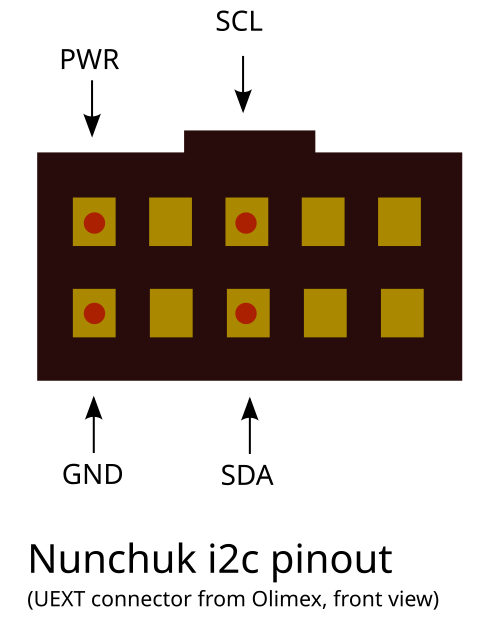
\includegraphics[width=0.3\textwidth]{common/nunchuk-pinout.pdf}\\
  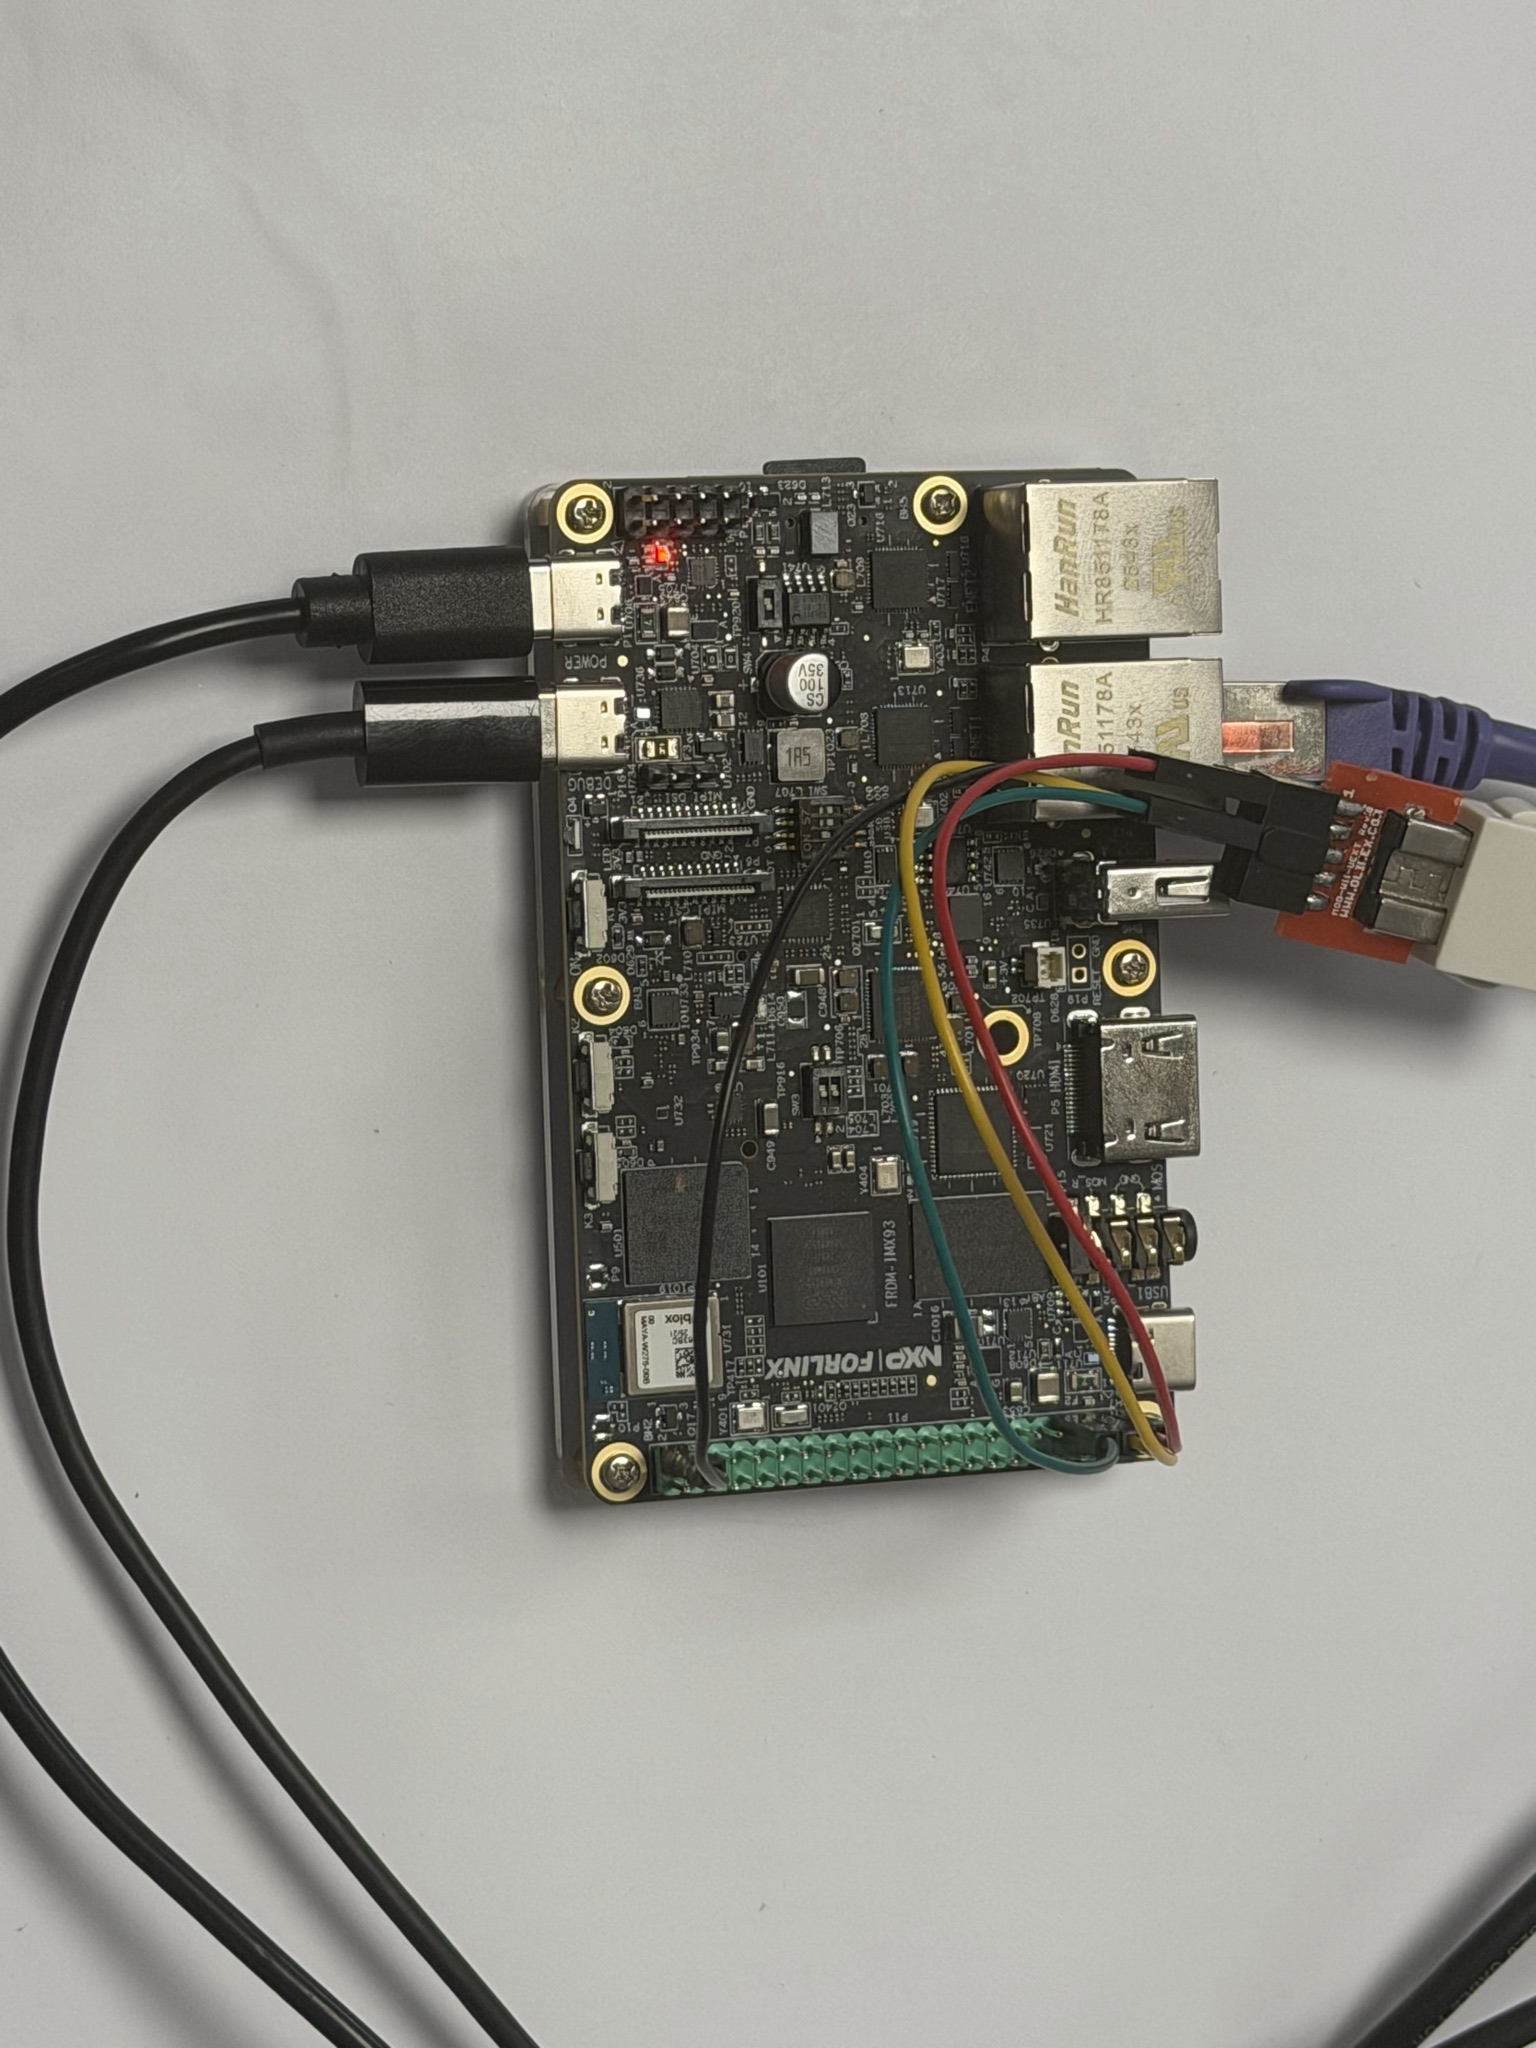
\includegraphics[width=0.5\textwidth]{labs/sysdev-accessing-hardware-imx93-frdm/imx93-frdm-connect-nunchuk.jpeg}
\end{center}

\begin{itemize}
\item Connect the Nunchuk PWR pin to \code{+3.3V} PIN 1 of the EXPI connector
\item Connect the Nunchuk GND pin to \code{GND} PIN 39 of the EXPI connector
\item Connect the Nunchuk SCL pin to \code{SCL} pin 5 of the EXPI connector
\item Connect the Nunchuk SDA pin to \code{SDA} pin 3 of the EXPI connector
\end{itemize}

If you didn't do any mistake, your new device should be detected at
address \code{0x52}:

\begin{verbatim}
# i2cdetect -r 3
i2cdetect: WARNING! This program can confuse your I2C bus
Continue? [y/N] y
     0  1  2  3  4  5  6  7  8  9  a  b  c  d  e  f
00:          -- -- -- -- -- -- -- -- -- -- -- -- --
10: -- -- -- -- -- -- -- -- -- -- -- -- -- -- -- --
20: -- -- -- -- -- -- -- -- -- -- -- -- -- -- -- --
30: -- -- -- -- -- -- -- -- -- -- -- -- -- -- -- --
40: -- -- -- -- -- -- -- -- -- -- -- -- -- -- -- --
50: -- -- 52 -- -- -- -- -- -- -- -- -- -- -- -- --
60: -- -- -- -- -- -- -- -- -- -- -- -- -- -- -- --
70: -- -- -- -- -- -- -- --
\end{verbatim}

We will later compile an out-of-tree kernel module to support this device.

\section{Plugging a USB audio headset}

In the next labs, we are going to play audio using a USB audio headset.
Let's see whether our kernel supports such hardware by plugging the
headset provided by your instructor.

Before plugging the device, look at the output of \code{lsusb}:

\begin{bashinput}
# lsusb
Bus 001 Device 001: ID 1d6b:0002 Linux 7.1.3 ehci_hcd EHCI Host Controller
\end{bashinput}

{\bf Known issue:} if you don't get any output from \code{lsusb},
you may need to remove the power supply and power on the board
again.

Now, when you plug the USB headset, a number of messages should appear
on the console, and running \code{lsusb} again should show an
additional device:

\begin{bashinput}
# lsusb
Bus 001 Device 001: ID 1d6b:0002 Linux 7.1.3 ehci_hcd EHCI Host Controller
Bus 001 Device 002: ID 1b3f:2008 GeneralPlus USB Audio Device
\end{bashinput}

The device of vendor ID \code{1b3f} and product ID \code{2008} has
appeared. Of course, this depends on the actual USB audio device
that you used.

The device also appears in \code{/sys/bus/usb/devices/}, in a
directory whose name depends on the topology of the USB bus. When the
device was plugged, one of the kernel messages was:

\begin{bashinput}
usb 1-1: new full-speed USB device number 2 using ci_hdrc
\end{bashinput}

So if we go in \code{/sys/bus/usb/devices/1-1}, we get the {\em
sysfs} representation of this USB device:

\begin{bashinput}
# cd /sys/bus/usb/devices/1-1
# cat idVendor
1b3f
# cat idProduct
2008
# cat manufacturer
GeneralPlus
# cat product
USB Audio Device
\end{bashinput}

However, while the USB device is detected, we currently do not have
any driver for this device, so no actual sound card is detected.

\section{Enabling, installing and using in-tree kernel modules}

Go back to the kernel source directory.

The Linux kernel has a generic driver supporting all USB audio devices
supporting the standard USB audio class. This driver can be enabled
using the \kconfig{CONFIG_SND_USB_AUDIO} configuration option. Look
for this parameter in the kernel configuration, you should find
it already enabled as a module.

So, instead of compiling the corresponding driver as a built-in, as
we did before, we'll take this good opportunity to practice with kernel modules.

So, compile your modules:
\begin{bashinput}
make modules
\end{bashinput}

Then, following details given in the lectures, install the modules in our NFS
root filesystem (\code{$HOME/__SESSION_NAME__-labs/tinysystem/nfsroot}).

Also make sure to update the kernel image (\code{make Image.gz}), and reboot the
board.  Indeed, due to the changes we have made to the kernel source code,
the kernel version is now \texttt{\workingkernel.<x>-dirty}, the {\em dirty}
keyword indicating that the Git working tree has uncommitted changes.
The modules are therefore installed in \texttt{/lib/modules/\workingkernel.<x>-dirty/},
and the version of the running Linux kernel must match this.

After rebooting, try to load the module that we need:

\begin{bashinput}
modprobe snd-usb-audio
\end{bashinput}

By running \code{lsmod}, see all the module dependencies that
were loaded too.

You can also see that a new USB device driver in
\code{/sys/bus/usb/drivers/snd-usb-audio}. This directory shows which
USB devices are bound to this driver.

You can check that \code{/proc/asound} now exists (thanks to loading
modules for ALSA, the Linux sound subsystem), and that one sound
card is available:

\begin{bashinput}
# cat /proc/asound/cards
 0 [Device         ]: USB-Audio - USB Audio Device
                      GeneralPlus USB Audio Device at usb-xhci-hcd.3.auto-1, full speed
\end{bashinput}

Check also the \code{/dev/snd} directory, which should now contain
some character device files. These will be used by the user-space
libraries and applications to access the audio devices.

Modify your startup scripts so that the \code{snd-usb-audio} module
is always loaded at startup.

We cannot test the sound card yet, as we will need to build some
software first. Be patient, this is coming soon.

\section{Compiling and installing an out-of-tree kernel module}

The next device we want to support is the I2C Nunchuk. There is a driver
in the kernel to support it when connected to a Wiimote controller, but
there is no such driver to support it as an I2C device.

Fortunately, one is provided in
\code{$HOME/__SESSION_NAME__-labs/hardware/data/nunchuk/nunchuk.c}. You can check
\href{https://bootlin.com/training/kernel/}{Bootlin's Linux kernel and
driver development course} to learn how to implement all sorts of device
drivers for Linux.

Go to this directory, and compile the out-of-tree module as follows:

\begin{bashinput}
make -C $HOME/__SESSION_NAME__-labs/kernel/linux M=$PWD
\end{bashinput}

Here are a few explanations:
\begin{itemize}
\item The \code{-C} option lets \code{make} know which Makefile to
      use, here the toplevel Makefile in the kernel sources.
\item \code{M=$PWD} tells the kernel Makefile to build external
      module(s) from the file(s) in the current directory.
\end{itemize}

Now, you can install the compiled module in the NFS root filesystem
by passing the \code{modules_install} target and specifying the
target directory through the \code{INSTALL_MOD_PATH} variable:

\begin{bashinput}
make -C $HOME/__SESSION_NAME__-labs/kernel/linux \
     M=$PWD \
     INSTALL_MOD_PATH=$HOME/__SESSION_NAME__-labs/tinysystem/nfsroot \
     modules_install
\end{bashinput}

You can see that this installs out-of-tree kernel modules under
\code{lib/modules/<version>/updates/}.

Back on the target, you can now check that your custom module can
be loaded:

\begin{bashinput}
# modprobe nunchuk
[ 4317.737978] nunchuk: loading out-of-tree module taints kernel.
\end{bashinput}

See \kdochtml{kbuild/modules} in kernel documentation
for details about building out-of-tree kernel modules.

However, run \code{i2cdetect -r 3} again. You will see that the
Nunchuk is still detected, but still not driven by the kernel.
Otherwise, it would be signaled by the \code{UU} character. You
may also look at the \code{nunchuk.c} file and notice a
\code{Nunchuk device probed successfully} message that you didn't
see when loading the module.

That's because the Linux kernel doesn't know about the Nunchuk
device yet, even though the driver for this kind of devices is
already loaded. Our device also has to be described in the Device Tree.

You can confirm this by having a look at the contents of the
\code{/sys/bus/i2c} directory.  It contains two subdirectories:
\code{devices} and \code{drivers}.

In \code{drivers}, there should be a \code{nunchuk} subdirectory,
but no symbolic link to a device yet. In \code{devices} you should
see some devices, but not the Nunchuk one yet.

\section{Declaring an I2C device}

To allow the kernel to manage our Nunchuk device, let's declare the
device in the custom Device Tree for our board. The declaration of the \busname\
bus will then look as follows:

\begin{verbatim}
&lpi2c4 {
        pinctrl-names = "default";
        pinctrl-0 = <&pinctrl_lpi2c4_expi>;
        status = "okay";
        clock-frequency = <100000>;

        nunchuk: joystick@52 {
                compatible = "nintendo,nunchuk";
                reg = <0x52>;
        };
};
\end{verbatim}

Here are a few notes:
\begin{itemize}
\item The \code{clock-frequency} property is used to configure the bus
      to operate at 100 KHz. This is supposed to be required for the
      Nunchuk.
\item The Nunchuk device is added through a child node in the I2C
      controller node.
\item For the kernel to {\em probe} and drive our device, it's required
      that the \code{compatible} string matches one of the
      \code{compatible} strings supported by the driver.
\item The \code{reg} property is the address of the device on the
      I2C bus. If it doesn't match, the driver will probe the device
      but won't be able to communicate with it.
\end{itemize}

Recompile your Device Tree and reboot your kernel with the new binary.

You can now load your module again, and this time, you should see that
the Nunchuk driver probed the Nunchuk device:

\begin{bashinput}
# modprobe nunchuk
[    7.638431] nunchuk: loading out-of-tree module taints kernel.
[    7.669813] input: Wii Nunchuk as /devices/platform/bus@f0000/42540000.i2c/i2c-3/3-0052/input/input2
[    7.679188] Nunchuk device probed successfully
\end{bashinput}

List the contents of \code{/sys/bus/i2c/drivers/nunchuk} once again. You
should now see a symbolic link corresponding to our new device.

Also list \code{/sys/bus/i2c/devices/} again. You should now see the
Nunchuk device, which can be recognized through its \code{0052} address.
Follow the link and you should see a symbolic link back to the Nunchuk
driver!

We are not ready to use this input device yet, but at least we can test
that we get bytes when buttons or the joypad are used. In the below
command, use the same number as in the message you got in the console
(\code{event2} for \code{input2} for example):

\begin{bashinput}
# cat /dev/input/event2 | od -x
\end{bashinput}

{\bf Caution}: using \code{od} directly on input event files should
work but is currently broken with the Musl library. We are investigating
this issue.

We will use the Nunchuk to control audio playback in an upcoming lab.

\section{Setting the board's model name}

Modify the custom Device Tree file one last time to override the model
name for your system. Set the \code{model} property to
\code{BeaglePlay media player}. Don't hesitate to ask your
instructor if you're not sure how.

Recompile the device tree, and reboot the board with it. You should see
the new model name in two different places:

\begin{itemize}
\item In the first kernel messages on the serial console.
\item In \code{/sys/firmware/devicetree/base/model}. This can be
      handy for a distribution to identify the device it's running on.
      By the way, you can explore \code{/sys/firmware/devicetree} and
      find that every subdirectory corresponds to a DT node, and every
      file corresponds to a DT property.
\end{itemize}

\section{Committing kernel tree changes}

Now that our changes to the kernel sources are over,
create a branch for your changes and create a patch for them.
{\bf Please don't skip this step} as we need it for the next labs.

First, if not done yet, you should set your identity
and e-mail address in git:

\begin{bashinput}
git config --global user.email "linus@bootlin.com"
git config --global user.name "Linus Torvalds"
\end{bashinput}

This is necessary to create a commit with the \code{git commit -s}
command, as required by the Linux kernel contribution guidelines.

Let's create the branch and the patch now:

\begin{bashinput}
git checkout -b bootlin-labs
git add arch/arm64/boot/dts/freescale/imx93-11x11-frdm-custom.dts
git commit -as -m "Custom DTS for Bootlin lab"
\end{bashinput}

We can now create the patch:\\
\texttt{git format-patch stable/linux-\workingkernel.y}

This should generate a \code{0001-Custom-DTS-for-Bootlin-lab.patch}
file.

Creating the branch will impact the versions of the kernel and the modules.
Compile your kernel and install your modules again (not necessary for the
Nunchuk one for the moment) and see the version changes through the
new base directory for modules.

To save space for the next lab, remove the old directory under
\code{lib/modules} containing the "dirty" modules.

Don't forget to update the kernel your board boots.

That's all for now!
